\definecolor{red}{rgb}{1,0,0}
\definecolor{green}{rgb}{0,0.39,0}
\renewcommand{\arraystretch}{1.1}

\subsection{Architecture}
\begin{frame}
\frametitle{RESNET-50}
\framesubtitle{Architecture (2015)} 

\begin{textblock}{15}(7.67,-0.62)
	\begin{figure}[H]
		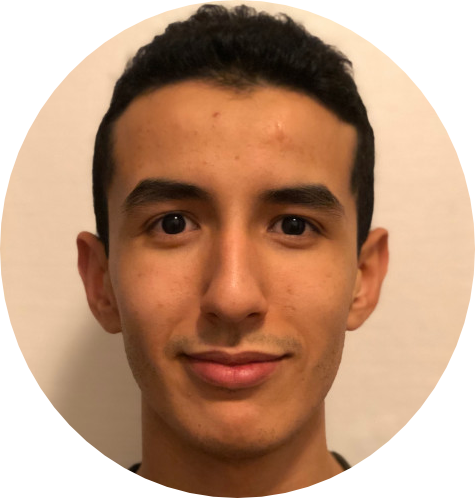
\includegraphics[width=0.1\textwidth]{Images/Team/MehdiABOUZAID.png} 
	\end{figure}
\end{textblock}

\begin{textblock}{1}(8.7,1)
	\centerline{50 trainable layers ; 25,636,712 parameters}
\end{textblock}

\begin{center}
	
	{\fontsize{7.5}{0}\selectfont
		\begin{tabular}{ccccc}
			
			\textbf{Layer} & \textbf{Type} & \textbf{Activation function} & \textbf{Output Shape} & \textbf{Param} \\
			input\_1  & (\textcolor{gray}{InputLayer}) & N/A & (224, 224, 3) & \colorbox{yellow}{0} \\             
			res..\_branch.. & (\textcolor{orange}{Conv2D}) & N/A & (112, 112, 64) & 9,472 \\    
			bn..\_branch.. & (\textcolor{red}{Batch Normalization}) & N/A & (112, 112, 64) & 256 \\     
			activation\_.. & (\textcolor{cyan}{Activation}) & ReLU & (112, 112, 64) & \colorbox{yellow}{0} \\
			max\_pooling2d\_1 & (\textcolor{blue}{MaxPooling2D}) & N/A & (56, 56, 64) & \colorbox{yellow}{0} \\     
			
			res..\_branch.. & (\textcolor{orange}{Conv2D}) & N/A & (56, 56, 64) &  4,160 \\ 
			bn..\_branch..  & (\textcolor{red}{Batch Normalization}) & N/A & (56, 56, 64) & 256 \\ 
			activation\_.. & (\textcolor{cyan}{Activation}) & ReLU & (56, 56, 64) & \colorbox{yellow}{0} \\
			res..\_branch.. & (\textcolor{orange}{Conv2D}) & N/A & (56, 56, 64) & 36,928 \\ 
			bn..\_branch..  & (\textcolor{red}{Batch Normalization}) & N/A & (56, 56, 64) & 256 \\          
			activation\_.. & (\textcolor{cyan}{Activation}) & ReLU & (56, 56, 64) & \colorbox{yellow}{0} \\
			res..\_branch.. & (\textcolor{orange}{Conv2D}) & N/A & (56, 56, 256) & 16,640 \\ 
			bn..\_branch..  & (\textcolor{red}{Batch Normalization}) & N/A & (56, 56, 256) & 256 \\ 
			activation\_.. & (\textcolor{cyan}{Activation}) & ReLU & (56, 56, 64) & \colorbox{yellow}{0} \\
			& ... & & &\\
			res..\_branch.. & (\textcolor{orange}{Conv2D}) & ReLU & (28, 28, 128) & 32,896 \\ 
			& ... & & &\\   
			res..\_branch.. & (\textcolor{orange}{Conv2D}) & ReLU & (28, 28, 128) & 147,584 \\         
			res..\_branch.. & (\textcolor{orange}{Conv2D}) & ReLU & (28, 28, 512) & 66,048 \\   
			
			res..\_branch.. & (\textcolor{orange}{Conv2D}) & ReLU & (14, 14, 256) & 131,328 \\   
			res..\_branch.. & (\textcolor{orange}{Conv2D}) & ReLU & (14, 14, 256) &  590,080  \\         
			res..\_branch.. & (\textcolor{orange}{Conv2D}) & ReLU & (14, 14, 1024) & 263,168 \\  
			
			res..\_branch.. & (\textcolor{orange}{Conv2D}) & ReLU & (7, 7, 512) & 524,800 \\   
			res..\_branch.. & (\textcolor{orange}{Conv2D}) & ReLU & (7, 7, 512) & 2,359,808 \\   
			res..\_branch.. & (\textcolor{orange}{Conv2D}) & ReLU & (7, 7, 2048) & 1,050,624 \\
			
			
			avg\_pool & (\textcolor{blue}{GlobalAveragePooling2D}) & N/A & (,2048) & \colorbox{yellow}{0} \\         
			fc1000 & (\textcolor{green}{Dense}) & SoftMax & (, 1000) & \colorbox{magenta}{2,049,000} \\ 
			
		\end{tabular}
	}
\end{center}
\end{frame}





\begin{frame}
\frametitle{RESNET-50}
\framesubtitle{Transfer Learning} 

\begin{textblock}{15}(7.67,-0.62)
\begin{figure}[H]
	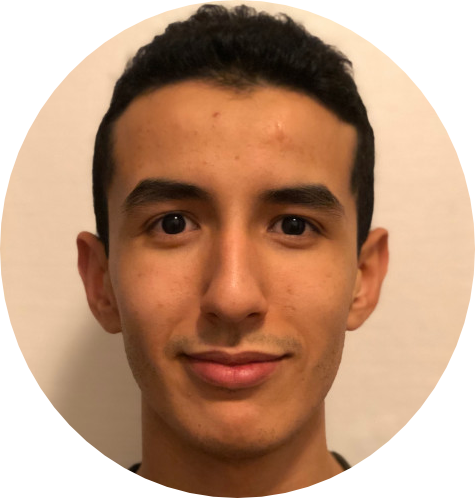
\includegraphics[width=0.1\textwidth]{Images/Team/MehdiABOUZAID.png} 
\end{figure}
\end{textblock}

\begin{center}
{\fontsize{8.5}{6.5}\selectfont
	\begin{tabular}{@{\hspace{-0.2cm}}cccc}
		& \textbf{Layer Type} &\textbf{Activation function} & \textbf{Output Shape} \\
		& & \textcolor{white}{phantom} & \\
		\begin{tabular}{c}
			freeze weights\\ learned on ImageNet
		\end{tabular}	
		& $\left\{\begin{tabular}{c}
		(\textcolor{gray}{InputLayer}) \\         
		(\textcolor{orange}{Conv2D}) \\      
		
		(\textcolor{blue}{MaxPooling2D}) \\         
		(\textcolor{orange}{Conv2D}) \\     
		(\textcolor{orange}{Conv2D}) \\             
		(\textcolor{orange}{Conv2D}) \\    
		(\textcolor{orange}{Conv2D}) \\    
		(\textcolor{orange}{Conv2D}) \\            
		(\textcolor{orange}{Conv2D}) \\   
		(\textcolor{orange}{Conv2D}) \\   
		(\textcolor{orange}{Conv2D}) \\        
		(\textcolor{orange}{Conv2D}) \\   
		(\textcolor{orange}{Conv2D}) \\  
		(\textcolor{orange}{Conv2D}) \\   
		(\textcolor{orange}{Conv2D})  \\   
		(\textcolor{blue}{GlobalAveragePooling2D})\\  
		\end{tabular}
		\right.\kern-\nulldelimiterspace$
		& \begin{tabular}{c}
			N/A \\
			ReLU \\
			ReLU \\
			ReLU \\
			ReLU \\
			ReLU \\
			ReLU \\
			ReLU \\
			ReLU \\
			ReLU \\
			ReLU \\
			ReLU \\
			ReLU \\
			ReLU \\
			ReLU \\
			ReLU \\
			ReLU \\	
		\end{tabular}
		& \begin{tabular}{c}
			(224,224,3) \\
			(112, 112, 64) \\
			(56, 56, 64) \\
			(56, 56, 64) \\
			(56, 56, 64) \\
			(56, 56, 256) \\
			(28, 28 , 128) \\
			(28, 28, 128) \\
			(28, 28, 512) \\
			(14, 14, 256) \\
			(14, 14, 256) \\
			(14, 14, 1024) \\ 
			(7, 7, 512) \\
			(7, 7, 512) \\
			(7, 7, 2048) \\
			(,2048)
		\end{tabular} \\
		& \hspace{0.2cm} \sout{(\textcolor{green}{Dense})} & \sout{\textcolor{red}{Softmax}} & \sout{(, 1000)} \\
		\only<2>{& \hspace{0.2cm} \textcolor{magenta}{(Dropout)} & N/A & (, 2048) \\} 
		train this layer & \hspace{-0.5cm} $\left\{\begin{tabular}{c}
		\hspace{0.5cm} (\textcolor{green}{Dense})
		\end{tabular} \right.\kern-\nulldelimiterspace$ & \textcolor{red}{Softmax} & \hspace{0.1cm} (, nbClasses)
	\end{tabular}
}
\end{center}
Trainable params: 6,147
\end{frame}
